\chapter{Formalizing Claims}
\label{chap:formalization}

In the previous chapter we have explored how to identify claims in text.
Now, we wish to lay the ground work for the next step: structuring those claims. 
To do so, we first need a model according to which the claims will be structured. 
Unlike most approaches in argumentation mining and computational argumentation that
assume a claim is atomic, we wish to disect claims by working on a 
sub-claim level. Our final goal is deriving a logical representation of a claim. 

Deriving the logical form of a natural language utterance is the task of
semantic parsing. Semantic parsing is divided into shallow and deep semantic parsing. 
Shallow semantic parsing (also denoted semantic role labeling) attempts to
identify entities in a text and assign roles to identified entities
\citep{pradhan2004shallow}. 
Deep semantic parsing deals with producing precise meaning representations
with complex (compositional) expressions \citep{pasupat2015compositional}. 
Semantic parsing is based on frame semantics, a theory of lingustic meaning
according to which one cannot understand the meaning of a single word without
all essential knowledge that relates to the word \citep{fillmore2006frame}.
A semantic frame can then be defined as a coherent structure of related concepts,
such that without knowledge of all of them, one does not have complete knowledge
of any one. An example semantic frames is ``buy'',  which is 
enriched with actor entities (``buyer'', ''seller'', etc.).
Formalizing claims is closely related to the task of semantic parsing, as the
goal is to derive a machine-understandable, logical representation of a claim.
However, claim formalization ``frames'' do not attempt to derive the exact
meaning of a claim, but reflect the argumentative structure of a claim. 
The argumentative structure of a claim should mainly involve the modality of the
claim speaker and the form of a claim (implication, contradiction). 

This chapter is divided into two main parts.  In the first part, the
microstructures are introduced (Section~\ref{sec:for_microstructures}).
Microstructures are based off on work described in \citep{boltuzic2017toward}.
In the second part (Section~\ref{sec:ontology_formalization}), we introduce a a
formalization based on ontologies. To demonstrate examples of both formalization
standards, we first take the dataset of claims and their respective paraphrases
described in Section~\ref{sec:claim_seg_data}. We then formalize claims 
according to the microstructure and ontology standard.

\section{Microstructures}
\label{sec:for_microstructures}

\begin{figure}
	\begin{center}
      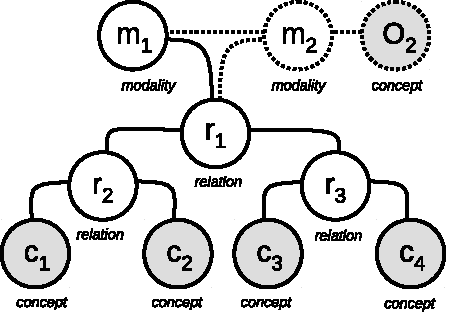
\includegraphics[scale=1]{microstructure.pdf}
      \end{center}
      \caption{Claim microstructure (2nd-order).}
  \label{fig:structures_flowchart}
\end{figure}

Microstructures are structures expressing relations between the domain-specific
concepts, reflecting beliefs, value judgements, or desired policies of the claim
author. Their purpose is to capture the gist of the claim. 
They were constructed in a data driven process
from many claims one could express as a \emph{relation}
between \emph{concepts} using a certain \emph{modality}. 
Figure~\ref{fig:structures_flowchart} shows a claim microstructure bringing three elements 
together. 

\paragraph{Relations. }  Many claims can be represented as expressing a
relation between two concepts. For example, on the topic of ``Gay Rights'', 
the relations may be `\texttt{promotes(gay marriage, depopulation)}' and 
`\texttt{purpose(love, procreation)}'. 
There are also comparably fewer claims that can be expressed via
higher-order relations , e.g. `\texttt{entails(constitution, allow(state, gay marriage))}. 
Each relation can be negated, e.g. $\neg$\texttt{promotes(gay marriage,
depopulation)} expresses that gay marriage does not cause depopulation. 
Relations are domain independent. 

\paragraph{Concepts. }
The relations are established between concepts, expressed by noun phrases. 
For ease of access, they can be arranged into a small, domain specific taxonomy of concepts. 
For instance ``gay marriage'', ``heterosexual marriage'' and ``religious marriage''
all belong under the concept of ``marriage''. 
The taxonomic relations could also be useful for later computational processing. 
Concepts are domain dependent and need to defined for each topic anew.

\paragraph{Modalities. }
We observe that claims are expressed under different modalities. 
They can be roughly categorized into \textit{beliefs, value judgements, and policies}. 
We formalize this via unary relations `believes', `approves', `disapproves',
and `desires' corresponding 
to beliefs (factual, religious, and opinion-based), positive value judgements, negative value 
judgements, and desired policy (desired state of affairs), respectively. 
The three modalities act as a wrapper on the propositional content of the claim, 
effectively modulating what is being claimed. 
For instance, `\texttt{believes(purpose(love, procreation))}' expresses the belief 
that love serves procreation, while \texttt{desires(}$\neg$\texttt{allow(state, gay marriage))}'
expresses the wish for the state not to allow gay marriages. 

\paragraph{Second opinion holder. }
Finally, in a number of claims the claim is expressed with a reference to a second
opinion holder (e.g. the Bible, the state). 
To tackle this, we add an additional modality layer with the opinion holder as
an additional modifier. 
For instance `\texttt{believes (believes[state] (promotes(marriage, advancement)))}' corresponds
to the belief that the state believes gay marriages lead to an advancement. 
By convention, the opinion holder of the first modality is always the author of the post. 

\begin{table}
{\footnotesize
\begin{tabular}{lp{0.80\columnwidth}}
\toprule
\textbf{Relation} & \textbf{Definition} \\
\midrule
\texttt{promotes(A, B)} & Promoting agent A promotes, fosters, leads, increases likelihood, boosts B.  \\
\texttt{suppress(A, B)} & Suppressing agent A suppresses, decreases likelihood, puts down, vanquishes B \\
\midrule
\texttt{allow(A, B)} & Principle A allows, approves, licenses state of affairs B \\
\midrule
\texttt{entails(A, B)} & State of affairs A, necessarily, per definition or causally, makes B true. \\
\texttt{contradicts(A, B)} & State of affairs A, necessarily, per definition or causally, makes B false. \\
\midrule
\texttt{purpose(A, B)} & The purpose of A is B. \\
\midrule
\texttt{equal(A, B)} & State of affairs A is equal to state of affairs B. \\
\midrule
\texttt{has(A, B)} & A has the properties affected by the existence of B.  \\
\bottomrule
\end{tabular}}
\caption{Relation types in claim microstructures.}
\label{tab:microstructures_relations}
\end{table}

\paragraph{Microstructure formalization. } Let $\mathcal{R}, \mathcal{C}$, and
$\mathcal{M}$ denote the set of relations, concepts and
modalities, respectively. 
Formally, we define a claim microstructure as a quadruple 
$$
(m_1, m_2, o_2, r)
$$ 
where $m_1 \in \mathcal{M}$, $m_2 \in \mathcal{M} \cup \{\epsilon\}$,
$o_2 \in \mathcal{C} \cup \{\epsilon\}$ is the optional second opinion holder, and 
$r = (t, c_1, c_2) \in \mathcal{R}$ is the (possibly higher order) relation 
between two concepts or relations $c_1, c_2 \in \mathcal{C} \cup \mathcal{R}$
conveyed by the relation type $t$.
Table~\ref{tab:microstructures_relations} lists all possible relation types. 
In Chapter~\ref{chap:analysis} we will show
how this microstructure formalization can be used. 
Now that we have formally defined microstructures, we move on to another
formal claim representation. 

\begin{table*}[t]
\begin{center}
{\footnotesize
	\begin{tabular}{@{}p{0.17\linewidth} p{0.25\linewidth} p{0.55\linewidth}@{}}
\toprule
\textbf{User post} & \textbf{Claim segment} & 
	%	\textbf{Claim paraphrase} & 
		\textbf{Claim microstructure}       \\
\midrule
\multirow{3}{*}{\parbox{2.6cm}{
		\emph{Men should fall in love with women that's why they where
		created and women should get married to men because it makes
		everything easier. }
}}
&  
\emph{Men should fall in love with women.}
%& \emph{People of opposite sex should fall in love.}
&
		\texttt{desires(entails(OppositeSex, FallingInLove))}
\\
\cmidrule{2-3}
& \emph{that's why they where created} 
	%	& \emph{Men and women are created to pair.}
 & 
		\texttt{believes(purpose(MenAndWomen, Procreation))}
 \\
\cmidrule{2-3}
& \emph{women should get married to men because it makes everything easier.} 
%		&  \emph{Heterosexual marriages make everything easier.}
 &
 \texttt{believes(entails(HeterosexualMarriage, Normal)) } \\
 \bottomrule
\end{tabular}}
\end{center}
\caption{An example of a user post segmented into three claim segments, each
	translated into the corresponding claim
	microstructure.}
\label{microstruc:tab:post_segments}
\end{table*}

\paragraph{Data annotation. }
We use the dataset defined in Chapter~\ref{chap:claim_segmentation}
and single out the ``\emph{Gay Rights}'' topic. We end with 100 
posts (50 \pro{pro} and 50 \con{con}), which break down into 920 claims and their
respective paraphrases. We ask two annotators (A1 and A2) to translate each of 
the 920 claims into claim microstructures. The annotators were provided 
with a domain-specific taxonomy on ``\emph{Gay Rights}'', compiled 
based on a manual analysis of claims. The taxonomy consists of 150 concepts
arranged into a tree of maximum depth of four. The annotators
were instructed to use the existing concepts from the taxonomy, and
introduce new ones only if they could not find a suitable one in the
taxonomy. They were also instructed not to use microstructures of order higher 
than two. Full annotation guidelines are listed in
Appendix~\ref{sec:microstructure_annotation_appendix}.
Out of 920 claims, annotator A1 managed to translate 882 claims into 707
distinct microstructures, while annotator A2 translated 842 claims into
767 distinct microstructures. The average annotation effort was 33 hours. 
The number of claims for which both provided an identical microstructure is only
58 (6.3\%). The annotators introduced 157 new concepts, indicating that the initial 
taxonomy was of too limited a scope. The low annotator agreement and relatively 
large number of added concepts suggest that a fair amount of ambiguity exists
in translating claims to microstructures. Our analysis revealed that, in the majority
of cases, the ambiguity is genuine and in such cases having more candidate 
microstructures for a single claim can be considered advantageous. 
The analysis also revealed that 'believes' is the most frequent modality, used for
79\% of the claims. For A1, \emph{entails} is the most common relation (61\%), while
A2 made a more balanced use of relations, with the top two being \emph{has} (21\%)
and \emph{entails} (15\%). The concepts most frequently used by A1 were
\emph{homosexuality}, \emph{homosexual people}, and \emph{marriage}, while for A2
these are \emph{the Bible}, \emph{homosexual people}, and \emph{government interest}. 
Example annotated microstructures are listed in Table~\ref{microstruc:tab:post_segments}. 

\section{Ontology-based formalization}
\label{sec:ontology_formalization}

Microstuctures provide a claim structure which can then be used 
to ``compress'' the claim for subsequent argumentation tasks
(see application to stance classification in Section~\ref{sec:stance_micro}).
However, microstructures do not inherently support any
well-established computer science standard. 
Hence, we turn to ontologies. Using ontologies not only allows for 
formalizing a claim, but also provides inference capabilities within
well-established frameworks (such as the resource description framework RDF). 

We propose an ontology-based framework ClaimOntology to formalize claims. The
ontology is key part of a formalization framework which defines how to
bootstrap a claim formalization from scratch. The end product of the framework
is an ontology containing formalized claims in a specific domain. 
The ontology itself is built on two levels: 
\begin{enumerate*}[label=(\arabic*)]
\item the upper and 
\item the domain ontology 
(the motivation behind using two-level ontologies in general is described in
		Section~\ref{sec:knowledge_representation}). 
\end{enumerate*}
The upper ontology formalizes abstract patterns in argumentative
claims as object properties. The domain-level ontology conceptualizes 
a specific discussion domain. The relationship between the upper 
and domain ontology is similar to a predicate-argument
relationship \citep{hindle1990noun}, where the upper ontology
defines argumentation-specific predicates --- defined through object properties, 
and the domain ontology defines arguments --- defined through 
individuals. 

The steps to be able to perform domain-specific claim analysis
involve
\begin{enumerate*}[label=(\arabic*)]
\item domain experts designing the domain ontology,
\item integrating the proposed domain ontology with the upper ontology,
\item defining the claims as individuals in the two-level ontology, and
\item validating claim individuals to ensure quality of fit for
	individuals in the domain ontology.
\end{enumerate*}
Completing these steps allows users of the formalization framework
to do deep domain claim analysis for the domain of interest. 
An example of a deep domain analysis can be found in Chapter~\ref{chap:analysis}.

Apart from modeling domain concepts and the relationships amongst them, we also
wish to formalize the \emph{type} of how the claim was expressed: as facts,
policies, and positive or negative value statements (see definition in
\citep{rieke1997argumentation} and microstructure
Section~\ref{sec:for_microstructures}). 

\subsection{ClaimOntology}
\label{subsec:claimontology}

\begin{figure}
	\centering
	\footnotesize
	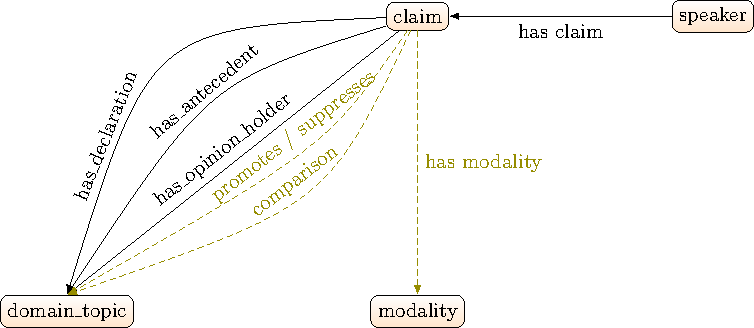
\includegraphics{formalizations_main_classes-figure0.pdf}
\caption{Main classes and properties of ClaimOntology. Dashed lines indicate
	semantic properties, full lines structural properties. 
	indicate. Arrow orientation indicates the
	triplet ordering. }
\label{fig:claimontology}
\end{figure}

The upper ontology represents general argumentation patterns, mostly on the
claim level.  The concepts and relations are used across different domains.
The central object of the upper ontology is the claim class. We are interested
in extracting as much as possible claims from a single topic. We leave the
levels above the claim (argument) is out of the thesis scope. The proposed ontology is an
OWL second-order description logic (2DL) ontology built using the
Prot\'{e}g\'{e} software \citep{gennari2003evolution}. The four main concepts
of the upper ontology are:
\begin{itemize}
	\item \texttt{claim}, corresponding to any argumentative statement,
	\item \texttt{speaker},  denoting the author of the claim
		(one speaker may be associated with $N$ \texttt{claims}),
	\item \texttt{type}, which is one of fact, value, or policy, and
	\item \texttt{domain\_topic}, representing any individual from the domain ontology.
\end{itemize}

The main concepts are related to each other through different types of object
properties, suitable to represent both the \emph{structural and semantic aspects} of
claims. The former aim at formalizing the structure of claims used in
the argumentation, such as the presence of an antecedent element. The latter
are used to describe the semantic relations in claims, for instance that
an element causes another one. Thus, on one hand, the attempt of 
formalizing structural aspects improves the analysis of structuring and
forming process of argumentation. On the other hand, this type of formalization
allows for a semantic analysis of building blocks, namely claims, used in 
argumentative discussions. Among the \emph{structural properties}, we identify:
\begin{itemize}
\item \texttt{has\_declaration}, 
\item \texttt{has\_antecedent},
\item \texttt{has\_opinion\_holder}, and
\item \texttt{has\_claim}. 
\end{itemize}
The \texttt{has\_declaration} property indicates an acknowledgement of
existence of a domain individual. For example, the claim 
\emph{marijuana consumption is out there} acknowledges
the existence of the domain individual \emph{marijuana consumption}.
The \text{has\_antecedent} property indicates the presence of an 
antecedent in a claim. The antecedent is always paired with some
form of a consequent, which is a semantic property. To indicate
there is a second opinion holder, the \texttt{has\_opinion\_holder}
property is used. The role of the \texttt{has\_opinion\_holder}
property is equivalent to the second opinion holder in the microstructure
formalization (see Section~\ref{sec:for_microstructures}). Finally, the speaker
who made the claim is attributed using the \texttt{has\_claim} property.

We discern between three different types of \emph{semantic properties}:
\begin{itemize}
\item \texttt{promotes / suppresses},
\item \texttt{comparison}, and
\item \texttt{has\_type}
\end{itemize}
The \texttt{promotes / suppresses} property is used to represent the claim
consequent as either a \texttt{promotes} or \texttt{suppresses} property
(inspired by \citet{hashimoto2012excitatory}). It is always paired with
the \texttt{has\_antecedent} structural property. The \texttt{promotes}
property has subproperties with \texttt{implies} and \texttt{causes}
properties, whereas the \texttt{suppresses} property has 
subproperties \texttt{contradicts} and \texttt{does\_not\_cause}.
The claim \texttt{claim\_x} made by \texttt{speaker\_x}
\emph{smoking marijuana hurts your lungs} can then be formalized as triplets:
\begin{align*}
	< & \mathit{claim\_x}, \hspace{0.1cm} \mathit{has\_antecedent}, \hspace{0.1cm}
	\mathit{marijuana\_consumption} > \\
	< & \mathit{claim\_x}, \hspace{0.1cm} \mathit{suppresses}, \hspace{0.1cm}
	\mathit{lung\_health} > 
\end{align*}
where \texttt{lung\_health} and \texttt{marijuana\_consumption} are 
domain individuals. 
Alternatively, it may also be formalized using different properties:
\begin{align*}
	< & \mathit{claim\_x}, \hspace{0.1cm} \mathit{has\_antecedent}, \hspace{0.1cm}
	\mathit{marijuana\_consumption} > \\
	< & \mathit{claim\_x}, \hspace{0.1cm} \mathit{causes}, \hspace{0.1cm}
	\mathit{lung\_damage} > 
\end{align*}
where \texttt{lung\_damage} is a domain individual. 
The \texttt{comparison} property is used to formalize a comparison of 
two domain concepts. There are three comparison object properties (each with the
\texttt{domain\_topic} as the object individual): \texttt{comparison\_greater},
\texttt{comparison\_less}, and \texttt{comparison\_criterion}. The
\texttt{comparison\_criterion} is optional and is used to denote the feature of 
comparison. For example, the claim \emph{alcohol is worse for your health than marijuana} can
be formalized as:
\begin{align*}
	< & \mathit{claim\_x}, \hspace{0.1cm} \mathit{comparison\_greater}, \hspace{0.1cm}
	\mathit{alcohol} > \\
	< & \mathit{claim\_x}, \hspace{0.1cm} \mathit{comparison\_less}, \hspace{0.1cm}
	\mathit{marijuana} >  \\
	< & \mathit{claim\_x}, \hspace{0.1cm} \mathit{comparison\_property}, \hspace{0.1cm}
	\mathit{health} > 
\end{align*}
The \texttt{has\_type} property reflects in which modality the claim was made. 
Claims \emph{marijuana should be legalized} and \emph{marijuana is legalized} 
can be formalized to have different types for the same domain concepts
(\emph{marijuana\_legalization}). 

The main classes and properties of ClaimOntology are visualized in 
Figure~\ref{fig:claimontology}. The domain ontology defines 
claim individuals as claims made by speakers of the
\texttt{domain\_individual} type. Thus, the domain individuals need to be
defined before making claim individuals. Now, we show a full formalization 
example on \emph{claim\_x} which states
\emph{heavy industry did not cause climate change}. Here, we may establish
two domain individuals: \texttt{industry} and \texttt{climate change}
connected via a \texttt{cause} property. Note that we omit the \emph{industry}
adjective \emph{heavy} which is a decision left to the domain expert to decide
on the granularity level of the domain ontology. 
More formally, we define \texttt{claim\_x} to contain properties:
\begin{align*}
	< & \mathit{claim\_x}, \hspace{0.1cm} \mathit{has\_antecedent}, \hspace{0.1cm}
	\mathit{industry} > \\
	< & \mathit{claim\_x}, \hspace{0.1cm} \mathit{does\_not\_cause}, \hspace{0.1cm}
	\mathit{climate\_change} >  \\
	< & \mathit{claim\_x}, \hspace{0.1cm} \mathit{has\_type}, \hspace{0.1cm}
	\mathit{fact} > 
\end{align*}

We define claims as done in Section~\ref{sec:claim_seg_data}, also 
abiding by nine principles. We reuse the claims and their paraphrases 
annotated in Section~\ref{sec:claim_seg_data} to formalize in ClaimOntology. 

\begin{algorithm}[t]
	\footnotesize{
	\begin{algorithmic}[1]
%\begin{Verbatim}[commandchars=\\\{\},codes={\catcode`$=3\catcode`_=8}]

\Function{viewpoint}{claim}
\State \begin{varwidth}[t]{\linewidth}
      map~$\gets$~"policy": "It should be that ", \par
        \hskip\algorithmicindent "good\_value": "I approve that ", \par
        \hskip\algorithmicindent "bad\_value": "I approve that ", \par
        \hskip\algorithmicindent "fact": ""
      \end{varwidth}

	\State 
	\Return map[claim.viewpoint]
	\State
\EndFunction
\State

\Function{negate}{claim, object}
\If{claim is\_negated}
\State
\Return " does not " + object
\Else
\State
\Return object
\EndIf

\EndFunction
\State

\If{claim.nprop == 1}
	\State object $\gets$ claim.property["has\_declaration"].object
	\State
	\Return viewpoint(claim) + negate(claim, object) + "exist"
\EndIf
\State
\If{claim.nprop == 2}
	\State ante $\gets$ claim.property["has\_antecedent"].object
	\State cons $\gets$ claim.property["promotes"].object
	\State
	\Return viewpoint(claim) + ante + negate(claim, object) + cons
\EndIf
\State
\If{claim.nprop == 3}
	\State less $\gets$ claim.property["comparison\_less"].object
	\State more $\gets$ claim.property["comparison\_greater"].object
	\State prop $\gets$ claim.property["comparison\_property"].object
	\State

	\State exp $\gets$ more + " is greater than " + less + " by " + prop
	\State
	\Return viewpoint(claim) + exp
\EndIf
\end{algorithmic}



% \textbf{function} viewpoint (claim)
%  map $\gets$ "policy": "It should be that ",
%         "good\_value": "I approve that ",
%         "bad\_value": "I disapprove that "
%         "fact": "
% \textbf{return} map[claim.viewpoint]
% 
% \textbf{function} negate (claim, object)
%   \textbf{if} claim is\_negated
%     \textbf{return} " does not " + object
%   \textbf{else} 
%     \textbf{return} object
%   \textbf{end if}
% 
% \textbf{if} claim.nary == 1
%   object = claim.property["has\_declaration"].object
%   \textbf{return} viewpoint(claim) + negate(claim, object) + "exist"
% 
% \textbf{if} claim.nary == 2
%   ante = claim.property["has\_antecedent"].object
%   cons = claim.property["promotes"].object
%   \textbf{return} viewpoint(claim) + ante + negate(claim, object) + cons
% 
% \textbf{if} claim.nary == 3
%   less = claim.property["comparison\_less"].object
%   more = claim.property["comparison\_greater"].object
%   prop = claim.property["comparison\_property"].object
% 
%   exp $\gets$ more + " is greater than " + less + " by " + prop
%   \textbf{return} viewpoint(claim) + exp
% \end{Verbatim}
}
\caption{Algorithm to generate a natural language sentence from a formalized
	claim individual. The claim \texttt{nprop} is the sum of how many object properties
	\texttt{has\_declaration}, \texttt{has\_antecedent}, \texttt{promotes}, 
	\texttt{comparison\_less}, \texttt{comparison\_greater}, \texttt{comparison\_property}
	does the claim contain}
\label{alg:formalization_to_sentence}
\end{algorithm}

To validate how well the formalized claims represent the original claims
made by the speakers, we propose measuring textual entailment between the formalized 
and the original claim. Textual Entailment (\textbf{TE}) models take a pair 
of sentences and predict whether the facts in the first sentence necessarily imply
facts in the second sentence (see Section~\ref{sec:textual_entailment} for a
a short introduction to textual entailment). Textual entailment expects 
sentences, so we have to translate the formalized claim back to natural language. 
For that purpose, we use Algorithm~\ref{alg:formalization_to_sentence}, which 
very roughly produces natural language sentences from formalizations. 
We acknowledge that produced sentences may not always be grammatical (depending on the
domain ontology). Using algorithm~\ref{alg:formalization_to_sentence} on the claim 
\texttt{claim\_y} with properties:
\begin{align*}
	< & \mathit{claim\_y}, \hspace{0.1cm} \mathit{comparison\_greater}, \hspace{0.1cm}
	\mathit{alcohol} > \\
	< & \mathit{claim\_y}, \hspace{0.1cm} \mathit{comparison\_less}, \hspace{0.1cm}
	\mathit{marijuana} >  \\
	< & \mathit{claim\_y}, \hspace{0.1cm} \mathit{comparison\_property}, \hspace{0.1cm}
	\mathit{mind\_influental} >  \\
	< & \mathit{claim\_y}, \hspace{0.1cm} \mathit{has\_type}, \hspace{0.1cm}
	\mathit{fact} > 
\end{align*}
produces the sentence \emph{alcohol is more than marijuana by being mind influental}.
Now, we compare this claim to the original and paraphrased claim via 
textual entailment models. Textual entailment estimates how well 
formalized claims represent original claims. To calculate
textual entailment between the (original or paraphrased) claim and reconstructed
formalized claim, we use the decomposable attention model \citep{parikh2016decomposable}
(available via Allennlp \citep{gardner2018allennlp}), which performs
close to the state-of-the-art on the widely used SNLI dataset \citep{bowman2015large}.

\subsection{Use-case: ``Marijuana'' }
\label{sec:usecase_ontology}

\begin{figure}
	\centering
	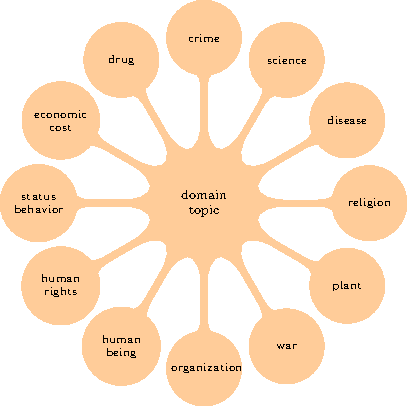
\includegraphics{formalizations_mindmap-figure0.pdf}
\caption{Marijuana legalization domain ontology top-level classes}
\label{fig:marijuana_domain_ontology}
\end{figure}

Now, we wish to apply the ClaimOntology to the ``\emph{Marijuana}'' topic in
two steps.  First, we construct a domain ontology ``\emph{Marijuana
legalization}''.  Second, we formalize claims from the ``\emph{Marijuana}''
topic as claim individuals. 

The domain ontology should contain domain specific classes, properties, and
instances. The idea is to build the domain ontology in a data driven 
fashion from speakers' claims. We build the domain ontology in two steps:
\begin{enumerate*}[label=(\arabic*)]
\item building the domain ontology of concepts, and 
\item claim individual annotation. 
\end{enumerate*}
After completing those two steps, the ontology can be used in a claim analysis. 

A domain ontology conceptualizes the specific domain of the online discussion. 
It is usually recommended to have some central terms around which to build
around (i.e., \emph{person}). We inspect claims in the ``\emph{Marijuana}'' topic,
using noun phrases as likely candidates for classes. We introduce
data properties mainly for noun phrases with some varying nuance relevant to
the domain. One example of using a data property would be to disambiguate between
\emph{illegal abortion} and \emph{legal abortion} by using boolean data
property \emph{legal} with the concept of \emph{abortion}.
Individuals of the domain ontologies should reflect all realizations of a concepts as
it appears in text. So, if we have a concept of \emph{taxes}, we require a concept
that covers all linguistic realizations in text, such as \emph{government tribute} or
\emph{compulsory state fee}. 

\begin{figure}
	\centering
	\footnotesize
	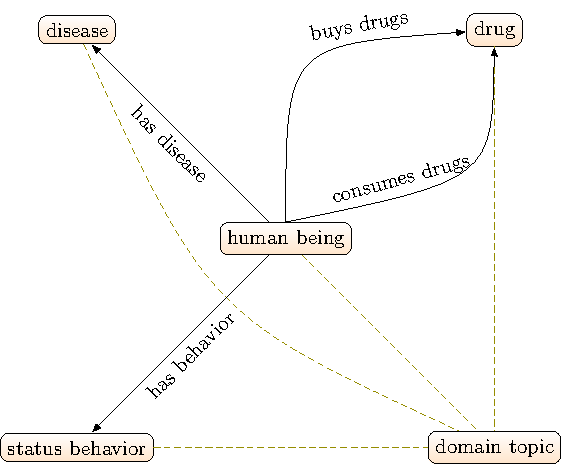
\includegraphics{formalizations_marijuana_main_classes-figure0.pdf}
\caption{Main classes and properties of the \textit{marijuana} domain 
ontology. 
Dashed lines indicate subclasses, full lines indicate object properties. 
The triple (\texttt{human\_being}, \texttt{buys\_drugs}, \texttt{drug}) represents an 
individual that belongs to the
\texttt{human\_being} class, which posses the property \texttt{buys\_drugs} with 
object \texttt{drug}.
} 
\label{fig:main-classes}
\end{figure}

The ``\emph{Marijuana legalization}'' domain ontology is built by experts over
several iterations with reviews in-between rounds. The end result proposes 
\texttt{domain\_topic} concepts, properties, and individuals. The 
domain ontology produced a diverse set of concepts, such as states (\texttt{war}),
people (\texttt{drug\_consumer}), or general abstract events (\texttt{society\_effect}). 
The top level classes of the ontology are displayed in 
Fig.~\ref{fig:marijuana_domain_ontology}. The relationships between some of the more frequently
used classes are shown in Fig.~\ref{fig:main-classes}. 
Individuals instantiate classes
and use properties. In total, 75 domain individuals were created, some of those
being \texttt{marijuana addicted consumer}, \texttt{legalized marijuana}, \texttt{
legalized alcohol}, \texttt{reduced mental capability}, etc. 
Fig.~\ref{fig:drug_domain_individuals} shows the hierarchy classes and 
individuals stemming from the drug class. 

\begin{figure}
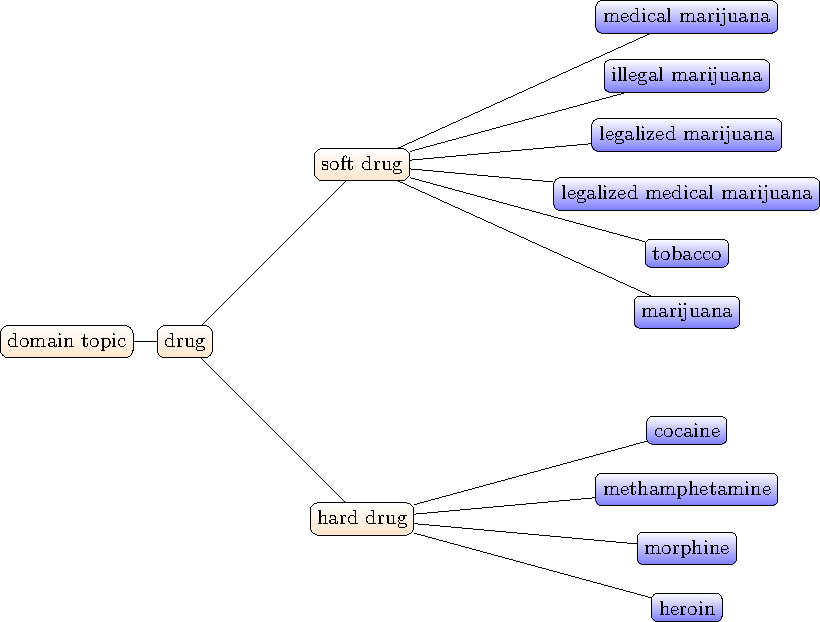
\includegraphics{formalizations_drug_hierarchy-figure0.pdf}
\caption{Marijuana legalization domain ontology drug individuals. 
	Classes/entities and orange and individuals are blue. }
	\label{fig:drug_domain_individuals}
\end{figure}


The ontology with domain individuals can now be merged with the upper ontology. 
Next, we move on to annotating claim individuals. Three expert annotators
formalize 920 claims from the ``\emph{Marijuana}'' topic. A few annotation
examples are listed in Table~\ref{tab:ontology_annotation}.
They fail to formalize 56, 53, and 60 claims, which makes about 6\% of the dataset. 
There are multiple reasons on why a claim is not suitable to be formalized. 
For one, a claim may be lacking appropriate domain individuals, such as in the claim
\emph{tobacco odors dissipate quickly}, where we \emph{tobacco odor} is a concept
not seen when building the domain individuals. Other non-formalized claims
deemed too abstract in meaning, an example being \emph{nothing can bring 
world peace}. In 243 out of 920 claims, the same formalization was produced 
by all three annotators, whereas for 325 two out of three annotators agreed. 
Upon manually checking formalizations at random, we observe that some
formalizations were different, yet equally suitable. After annotating and manually
checking claim individuals, we move on to  automatic validation. 

\begin{table*}[t]
	\begin{tabular}{p{5cm}|p{5cm}|p{5cm}}
	\toprule
Original & Paraphrased & Formalized \\
\midrule
Pot hurts you & Marijuana is bad for your health & Marijuana consumption has negative health effects \\

One may suffer or develop hallucinations, &                                                                                            
When one is under the influence of marijuana, one may hallucinate. &       
marijuana consumer causes mind influential \\ 

Cannabis has been proven to have health benefits . & 
Marijuana has been proven to have health benefits. & 
marijuana suppresses negative health effect \\

legalization would open up a larger market for vaporizers, &                                                                                          
Legalizing marijuana would open up a larger market for vaporizers. &                                           
legalized marijuana promotes free market marijuana seller \\

YOU WILL DIE IF YOU USE THIS TO OFTEN &                                                                     
Using marijuana too often causes death. &                                                                                                                                                     
marijuana consumer promotes death \\                                                         
\bottomrule
\end{tabular}
\caption{Annotation examples. Original represents the unedited speakers' claim.
	Paraphrased represents the from canonical claim made by the annotators.
	Formalized is the text version  of the formalized claim (obtained by
	applying Algorithm~\ref{alg:formalization_to_sentence} on a formalized
	claim)
	}
\label{tab:ontology_annotation}
\end{table*}

With the domain ontology built and integrated with the upper ontology and claim
individuals annotated, it is considered a good practice to verify and validate
the resulting ontology. 
We first verify the ontology using Prot\'{e}g\'{e} to ensure logical
consistency. For validity, we estimate how much do formalized claims entail 
speakers' original claims by measuring textual entailment between the formalized
and original (or paraphrased) claim. 
Now, we compare formalized sentences to paraphrased claims, excluding 169 claims 
which at least one of the annotators deemed unsuitable to formalize. 
We use an off-the-shelf entailment system which outputs a decision $d \in \{E, C, N\}$
along with normalized decision probabilities, where $E$ stands for entailment, 
$C$ stands for contradiction, and $N$ for neutral (neither an entailment or 
contradiction relation hold). Since entailment is not a symmetric relation, we
measure by setting the claim as both the text and hypothesis. 

Measuring entailment across all three annotators, we observe 2591 pairs of claims
and formalizations. The entailment decision was made in 1323 (51\%), 1031 (40\%)
were neutral, and contradiction was found in the fewest number of pairs, 
237 (9\%). We compare this a randomized baseline where claims were 
paired with a randomly selected formalized claim. 
We obtain that the entailment decision was made in 
35\% of the cases in the randomized baseline. 
%TODO add numbers for random decisions
We manually inspect some of the examples to determine why were some 
pairs labelled as contradictions or neutral. 
% TODO add examples on false positives
Since the evaluation showed entailment decisions in 
15\% percent more 
than the randomized baseline, and that the contradiction-labelled examples 
seem to be hard to capture by the entailment system, we feel confident for this ontology
to pass the entailment validation step. 

% \section{Discussion}
% \label{sec:formalization_conclusion}
% 
% In this chapter, we proposed two formalizations for argumentative claims.  The
% first, microstructures define a domain dependent taxonomy of concepts and
% define relations amongst concepts. We annotate 920 claims from the ``\emph{Gay
% Rights}'' topic. A high number of claims (93\%) was successfully translated to
% microstructures.  However, it showed that two annotators managed to produce the
% identical microstructure in only 58 (6.3\%) cases in addition to introducing
% 157 new concepts. Although some of the differences can be attributed to
% microstructure ambiguity, this inter-annotator agreement rate is considered
% very low. 
% The second proposed formalization is based on ontologies. 
% The ontology formalization, ClaimOntology is built from an upper and 
% domain ontology. We annotate 920 claims from the ``\emph{Marijuana}''
% topic. Similarly to microstructures, a high number (94\%) of the dataset of
% successfully formalized.
% But, unlike microstructures, inter-annotator agreement was much higher, with 
% 61\% of claims having at least two identical formalizations. 

Microstructure and ontology formalizations represent first steps towards
sub-claim formalizations. Both model the linguistic argumentation patterns
joined with the the domain knowledge.  Having formalized claims will allow us
various applications in argumentation mining. In Chapter~\ref{chap:analysis},
we will use microstructures in stance classification, and claim ontologies to
deriving implicit claims.  Additionally, in
Chapter~\ref{chap:claim_structuring} we will explore how feasible it is to
automatically acquire formalized claims directly from text.  
